\documentclass[11pt]{article}
\usepackage{graphicx}
\usepackage[euler-digits]{eulervm}
\usepackage{charter,amsmath,amssymb,breakurl}
\usepackage[letterpaper,margin=1in]{geometry}
\usepackage{multicol}
\everymath{\displaystyle}
\author{}\date{Due in class Friday 20 February}
\title{Math 104 Written Assignment 4}\author{}
\begin{document}
\maketitle
\thispagestyle{empty}
\begin{enumerate}
\item
\begin{multicols}{2}
Having resolved to paint the rooms of your apartment
Aqua Sparkle, Galactica, and Kingston Aqua,
shown in the swatch at the right, you need to decide which color
to paint your living room, bedroom, and bathroom.
Since the living room adjoins the bedroom, those rooms should
be painted different colors. Similarly, since
the bedroom and the bathroom adjoin one another,
those rooms should also be painted different colors.
\begin{center}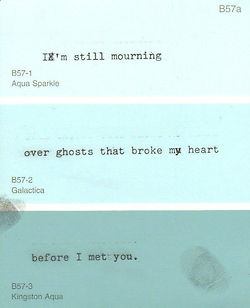
\includegraphics[scale=.5]{Swatch}\end{center}
\end{multicols}
\begin{enumerate}
\item Draw a tree diagram illustrating all the possible ways
to paint your apartment.
\item In how many ways can the project be realized?
\item What is the probability that Aqua Sparkle will be used in some room?
\item What is the probability that Galactica will be used more than one room?
\item In how many ways are all three colors used?
\end{enumerate}

\item When eating in an Indian restaurant with one other person,
I recommend that you order two different vegetable dishes,
a legume dish, and a starchy
dish. Below is the menu at an Indian restaurant.
\begin{center}\begin{tabular}{c|c|c}
\bf Vegetable&\bf Legume&\bf Starchy\\\hline
Alu gobi&Chana&Nan\\
Bharta&Dal&Rice\\
Sag
\end{tabular}\end{center}
However, if Dal is selected, then rice should also be selected
due to the runny nature of Dal.
\begin{enumerate}
\item Draw a tree diagram illustrating all the
possible meals that can be assembled from this
menu using my guidelines.
\item In how many ways can a meal be selected?
\item What is the probability that rice will be selected?
\item What is the probability that Alu Gobi will be selected?
\item In how many possibilities does Nan appear?
\end{enumerate}
\end{enumerate}
\end{document}
